\section{Concentration of Sums of Independent Random Variables}

\subsection{Why Concentration Inequalities?}
From previous chapters, the simplest concentration inequality is Chebyshev's Inequality, which is quite 
general but the bounds can often can be too weak. We can look at the following example:

\begin{example}
\label{ex:2.1.1}
Toss a fair coin $N$ times. What is the probability that we get at least $\frac{3}{4}$ heads?

Let $S_N$ denote the number of heads, then $S_N \sim \text{Binom}(N, \frac{1}{2})$. We get 
\[ \mathbb{E}[S_N] = \frac{N}{2}, \mathrm{Var}(S_n) = \frac{N}{4}. \]
Using Chebyshev's Inequality, we get 
\[ P(S_N \geq \frac{3}{4}N) \leq P(\bigg| S_N - \frac{N}{2} \bigg| \geq \frac{N}{4}) \leq \frac{4}{N}. \]
This means probabilistic bound from above converges linearly in $N$. 

However, by using the Central Limit Theorem, we get a very different result: If we let $S_N$ be a sum of 
independent $Be(\frac{1}{2})$ random variables. Then by the De Moivre-Laplace CLT, the random variable 
\[ Z_N = \frac{S_N - N/2}{\sqrt{N/4}} \]
converges to the standard normal distribution $N(0, 1)$. Then for a large $N$, 
\[ P(S_N \geq \frac{3}{4}N) = P(Z_N \geq \sqrt{N/4}) \approx P(Z \geq \sqrt{N/4}) \]
where $Z \sim N(0, 1)$. We will use the following proposition: 

\begin{proposition}[Gaussian tails]
\label{prop:2.1.2}
Let $Z \sim N(0, 1)$. Then for all $t > 0$, 
\[  \frac{t}{t^2 + 1} \cdot \frac{1}{\sqrt{2 \pi}}e^{-t^2 / 2} \leq P(Z \geq t) 
\leq \frac{1}{t} \cdot \frac{1}{\sqrt{2 \pi}}e^{-t^2 / 2}. \]
\end{proposition}

\begin{proof}
The first inequality is proved in exercise 2.2. For the second inequality, by making the change 
of variables $x = t + y$,
\begin{align*}
	P(Z \geq t) 
	&= \frac{1}{\sqrt{2 \pi}} \int_{t}^{\infty} e^{-x^2 / 2} \ dx \\
	&= \frac{1}{\sqrt{2 \pi}} \int_{0}^{\infty} e^{-t^2 / 2} e^{-ty} e^{-y^2 / 2} \ dy \\
	&\leq \frac{1}{\sqrt{2 \pi}} e^{-t^2 / 2} \int_{0}^{\infty} e^{-ty} \ dy 
	\quad (e^{-y^2 / 2} \leq 1) \\
	&= \frac{1}{t} \cdot \frac{1}{\sqrt{2 \pi}}e^{-t^2 / 2}.
\end{align*}
\end{proof}

Therefore the probability of having at least $\frac{3}{4}N$ heads is bounded by 
\[ \frac{1}{\sqrt{2 \pi}}e^{-N / 8}, \]
which is much better than the linear convergence we had above. However, this reasoning is not rigorous, 
as the approximation error decays slowly, which can be shown via the CLT below: 

\begin{theorem}[Berry-Esseen CLT]
Let $X_1, X_2, \dots$ be a sequence of i.i.d. random variables with mean $\mu$ and variance 
$\sigma^2$, and let $S_N = X_1 + Part of negotiations.\cdots + X_N$, and let 
\[ Z_N = \frac{S_N - \mathbb{E}[S_N]}{\sqrt{\mathrm{Var}(S_N)}}. \]
Then for every $N \in \mathbb{N}$ and $t \in \mathbb{R}$ we have 
\[ |P(Z_N \geq t) - P(Z \geq t)| \leq \frac{\rho}{\sqrt{N}}, \]
where $Z \sim N(0, 1)$ and $\rho = \mathbb{E}[|X_1 - \mu|^3] / \sigma^3$.
\end{theorem}
Therefore the approximation error decays at a rate of $1 / \sqrt{N}$. Moreover, this bound cannot be improved, 
as for even $N$, the probability of exactly half the flips being heads is 
\[ P(S_N = \frac{N}{2}) = 2^{-N} \binom{N}{N/2} \approx \sqrt{\frac{2}{\pi N}}. \]
where the last approximation uses Stirling approximation.

All in all, we need theory for concentration which bypasses the Central Limit Theorem.
\end{example}


\subsection{Hoeffding Inequality}
\begin{definition}[]
A random variable $X$ has the \underline{Rademacher Distribution} if it takes values $-1$ and $1$ 
with probability $1/2$ each, i.e. 
\[ P(X = -1) = P(X = 1) = \frac{1}{2}. \]
\end{definition}

\begin{theorem}[Hoeffding Inequality]
\label{thm:2.2.2}
Let $X_1, \dots, X_N$ be independent Rademacher random variables, and let $a = (a_1, \cdots, a_n) 
\in \mathbb{R}^n$ be fixed. Then for any $t \geq 0$, 
\[ P \biggl( \sum_{i = 1}^{N} a_iX_i \geq t \biggr) \leq \exp{\biggl( -\frac{t^2}{2\|a\|_2^2} \biggr)}. \]
\end{theorem}

\begin{proof}
The proof comes by a method called the \textit{exponential moment method}. We multiply the probability of 
the quantity of interest by $\lambda \geq 0$ (whose value will be determined later), exponentiate, 
and then bound using Markov's inequality, which gives: 
\begin{align*}
	P \biggl( \sum_{i = 1}^{N} a_iX_i \geq t \biggr) 
	&= P \biggl( \lambda \sum_{i = 1}^{N} a_iX_i \geq \lambda t \biggr) \\
	&= P \biggl( \exp{\biggl( \lambda \sum_{i = 1}^{N} a_iX_i \biggr)} \geq \exp{(\lambda t)} \biggr) \\
	&\leq e^{-\lambda t} \mathbb{E} \biggl[ \exp{\biggl( \lambda \sum_{i = 1}^{N} a_iX_i \biggr)} \biggr].
\end{align*}
In fact, from the last quantity we got above, we are effectively trying to bound the moment generating 
function of the sum $\sum_{i = 1}^{N} a_iX_i$. Since the $X_i$'s are independent, 
\[ \mathbb{E} \biggl[ \exp{\biggl( \lambda \sum_{i = 1}^{N} a_iX_i \biggr)} \biggr] 
= \prod_{i = 1}^{N} \mathbb{E}[\exp{(\lambda a_i X_i)}]. \]
Let's fix $i$. Since $X_i$ takes values $-1$ and $1$ with probability $1/2$ each, 
\[ \mathbb{E}[\exp{(\lambda a_i X_i)}] = \frac{1}{2}\exp{(\lambda a_i)} 
+ \frac{1}{2}\exp{(-\lambda a_i)} = \cosh{(\lambda a_i)}. \]
Next we will use the following inequality: 
\[ \cosh{x} \leq e^{x^2/2} \quad \text{for all } x \in \mathbb{R}. \]
The above is true by expanding the taylor series for both functions (proven in Exercise 2.5). Then 
we get 
\[ \mathbb{E}[\exp{(\lambda a_i X_i)}] \leq \exp{(\lambda^2 a_i^2 / 2)}. \]
Substituting this inequality into what we have above gives 
\begin{align*}
	P \biggl( \sum_{i = 1}^{N} a_iX_i \geq t \biggr) 
	&\leq e^{-\lambda t} \prod_{i = 1}^{N} \exp{(\lambda^2 a_i^2 / 2)} \\
	&= \exp{\biggl( -\lambda t + \frac{\lambda^2}{2}\sum_{i = 1}^{N} a_i^2 \biggr)} \\
	&= \exp{\biggl( -\lambda t + \frac{\lambda^2}{2} \|a\|_2^2 \biggr)}.
\end{align*}
Now we want to find the optimal value of $\lambda$ to make the quantity on the RHS as small as possible. 
Define the RHS as a function of $\lambda$,  and taking derivatives with respect to $\lambda$ yields
\[ f'(\lambda) = (-t + \lambda \|a\|_2^2) 
\exp{\biggl( -\lambda t + \frac{\lambda^2}{2} \|a\|_2^2 \biggr)} = 0 
\implies \lambda^* = \frac{t}{\|a\|_2^2}. \]
Then the second derivative test gives 
\[ f''(\lambda^*) = \|a\|_2^2 \exp{\biggl( -\lambda t + \frac{\lambda^2}{2} \|a\|_2^2 \biggr)} \geq 0. \]
Therefore the quantity is indeed minimized at $\lambda^*$, then plugging this value back gives 
\[ P \biggl( \sum_{i = 1}^{N} a_iX_i \geq t \biggr) 
\leq \exp{\biggl( -\frac{t^2}{2\|a\|_2^2} \biggr)}. \]
\end{proof}

\begin{remark}[Exponentially light tails]
Hoeffding inequality can be seen as a concentrated version of the CLT. With normalization $\|a\|_2 = 1$, 
we get an exponentially light tail $e^{-t^2 / 2}$, which is comparable to \cref{prop:2.1.2}.
\end{remark}

\begin{remark}[Non-asymptotic theory]
Unlike the classical limit theorems, Hoeffding inequality holds for every fixed $N$ instead of letting 
$N \to \infty$. Non-asymptotic results are very useful in data science because we can use $N$ as the 
sample size.
\end{remark}

\begin{remark}[The probability of $\frac{3}{4}N$ heads]
Using Hoeffding, returning back to \cref{ex:2.1.1} and bound the probabiltiy of at least $\frac{3}{4}N$ 
heads in $N$ tosses of a fair coin. Since $Y \sim \text{Bernoulli}(1/2)$, $2Y - 1$ is Rademacher. Since 
$S_N$ is a sum of $N$ independent $\text{Be}(1/2)$ random variables, $2S_N - N$ is a sum of $N$ 
independent Rademacher random variables. Hence 
\begin{align*}
	P(\text{At least } \frac{3}{4}N \text{ heads}) 
	&= P(S_N \geq \frac{3}{4}N) \\
	&= P(2S_N - N \geq \frac{N}{2}) \\
	&\leq e^{-N/8}.
\end{align*}
This is a rigorous bound comparable to what we had heuristically in the example.
\end{remark}

Hoeffding inequality can also be extended to two-sided tails and only suffers by a constant multiple 
of 2: 
\begin{theorem}[Hoeffding inequality, two-sided]Let $X_1, \dots, X_N$ be independent Rademacher random 
variables, and let $a = (a_1, \cdots, a_n) \in \mathbb{R}^n$ be fixed. Then for any $t \geq 0$, 
\[ P \biggl( \bigg| \sum_{i = 1}^{N} a_iX_i \bigg| \geq t \biggr) 
\leq 2\exp{\biggl( -\frac{t^2}{2\|a\|_2^2} \biggr)}. \]
\end{theorem}

\begin{proof}
Denote $S_N = \sum_{i = 1}^{N} a_iX_i$. By using the union bound,
\begin{align*}
	P(|S_N| \geq t) 
	&= P(S_N \geq t \cup S_N \leq -t) \\
	&\leq P(S_N \geq t) + P(-S_N \geq t).
\end{align*}
Then applying the exact process (exponential moment method) from above gives the result.
\end{proof}

Hoeffding inequality can be also be applied to general bounded random variables: 
\begin{theorem}[Hoeffding inequality for bounded random variables]
Let $X_1, \dots, X_N$ be independent random variables such that $X_i \in [a_i, b_i]$ for every $i$. Then 
for any $t > 0$, we have 
\[ P \biggl( \sum_{i = 1}^{N} (X_i - \mathbb{E}[X_i]) \geq t \biggr) 
\leq \exp{\biggl( -\frac{2t^2}{\sum_{i = 1}^{N} (b_i - a_i)^2} \biggr)}. \]
\end{theorem}

\begin{proof}
Done in Exercise 2.10.
\end{proof}


\subsection{Chernoff Inequality}
In general, Hoeffding inequality is good for Rademacher random variables, but it does not account for, say, 
the parameter $p_i$ within a Bernoulli random variable, which can lead to very different results depending 
on what this value is.

\begin{theorem}[Chernoff inequality]
\label{thm:2.3.1}
Let $X_i \sim \text{Ber}(p_i)$ be independent.Let $S_N = \sum_{i = 1}^{N} X_i$ and $\mu = \mathbb{E}[S_N]$. 
Then 
\[ P(S_N \geq t) \leq e^{-\mu} \biggl( \frac{e \mu}{t} \biggr)^t \quad \text{for any } t \geq \mu. \]
\end{theorem}

\begin{proof}
We'll use the exponential moment method as from \cref{thm:2.2.2} again. Fix $\lambda > 0$.
\begin{align*}
	P(S_n \geq t) 
	&= P(\lambda S_N \geq \lambda t) \\
	&= P(\exp{(\lambda S_n)} \geq \exp{(\lambda t)}) \\
	&\leq e^{-\lambda t} \mathbb{E}[\exp{(\lambda S_n)}] \\
	&= e^{-\lambda t} \prod_{i = 1}^{N} \mathbb{E}[\exp{(\lambda X_i)}]. 
\end{align*}
Fix $i$. Since $X_i \sim \text{Ber}(p_i)$, 
\[ \mathbb{E}[\exp{(\lambda X_i)}] = e^{\lambda} p_i + 1(1 - p_i) 
= 1 + (e^\lambda - 1)p_i \leq e^{\lambda - 1} p_i \]
where the last inequality comes from $1 + x \leq e^x$. So 
\[ \prod_{i = 1}^{N} \mathbb{E}[\exp{(\lambda X_i)}] \leq \exp{ \biggl( 
(e^\lambda - 1) \sum_{i = 1}^{N} p_i \biggr)} = \exp{((e^\lambda - 1)\mu)}. \]
Substituting back to the original equation gives 
\[ P(S_N \geq t) \leq e^{-\lambda t} \exp{((e^\lambda - 1)\mu)} 
= \exp{(-\lambda t + (e^\lambda - 1)\mu)}. \]
As before, define the above as a function of $\lambda$ and using calculus, 
\[ f'(\lambda) = (-t + \mu e^\lambda)\exp{(-\lambda t + (e^\lambda - 1)\mu)} = 0 
\implies \lambda^* = \ln{(t / \mu)}. \]
Moreover, 
\[ f''(\lambda^*) = t\exp{(-t \ln{(t / \mu)} + (t / \mu - 1)\mu)} \geq 0. \]
Therefore we have found the $\lambda^*$ that produces the tightest bound, and plugging back into the 
original equation gives the result.
\end{proof}

\begin{remark}[Chernoff inequality: left tails]
\label{rmk:2.3.2}
There is also a version of the Chernoff inequality for left tails: 
\[ P(S_N \leq t) \leq e^{-\mu} \biggl( \frac{e \mu}{t} \biggr)^t \quad \text{for every } 
0 < t \leq \mu. \]
\end{remark}

\begin{proof}
Done in Exercise 2.11.
\end{proof}

\begin{remark}[Poisson tails]
\label{rmk:2.3.3}
When $p_i$ is small for the Bernoulli random variables, by the Poisson Limit Theorem (add link), 
$S_N \sim \text{Pois}(\mu)$. Using Stirling approximation for $t!$, 
\[ P(S_N = t) \approx \frac{e^{-\mu}}{\sqrt{2 \pi t}} \biggl( \frac{e \mu}{t} \biggr)^t, 
\quad t \in \mathbb{N}. \]
Chernoff inequality gives a similar result, but rigorous and non-asymptotic. It is saying that we can 
bound a whole Poisson tail $P(S_N \geq t)$ by just one value $P(S_N = t)$ in the tail :)
\end{remark}

Poisson tails decay at the rate of $t^{-t} = e^{-t \ln{t}}$, which is not as fast as Gaussian tails. 
However, the corollary below shows that for small deviations, the Poisson tail resembles the Gaussian: 
\begin{corollary}[Chernoff inequality: small deviations]
In the setting of \cref{thm:2.3.1}, 
\[ P(|S_N - \mu| \geq \delta \mu) \leq 2 \exp{\biggl( -\frac{\delta^2 \mu}{3} \biggr)} \quad 
\text{for every } 0 \leq \delta \leq 1. \]
\end{corollary}

\begin{proof}
Using \cref{thm:2.3.1} with $t = (1 + \delta)\mu$, 
\begin{align*}
	P(S_N \geq (1 + \delta)\mu) \\
	&\leq e^{-\mu} \biggl( \frac{e \mu}{(1 + \delta)\mu} \biggr)^{(1 + \delta)\mu} \\
	&= e^{-\mu + (1 + \delta)\mu} \cdot e^{-\ln{(1 + \delta)} \cdot (1 + \delta)\mu} \\
	&= \exp{(-\mu((1 + \delta)\ln{(1 + \delta)} - \delta))}.
\end{align*}
Expanding the expression inside the exponent via Taylor series, 
\[ (1 + \delta)\ln{(1 + \delta)} - \delta = \frac{\delta^2}{2} - \frac{\delta^3}{2 \cdot 3} 
+ \frac{\delta^4}{3 \cdot 4} - \frac{\delta^5}{4 \cdot 5} + \cdots \geq \frac{\delta^2}{3}. \]
The last inequality is true because when we subtract $\delta^2 / 3$ on both sides, we get 
\[ \frac{\delta^4}{3 \cdot 4} - \frac{\delta^5}{4 \cdot 5} + \frac{\delta^6}{5 \cdot 6} - \cdots \geq 0 \]
because it is an alternating series with decreasing terms and a positive first term. Plugging the bound 
above into our first equation gives 
\[ P(S_N \geq (1 + \delta)\mu) \leq \exp{\biggl( -\frac{\delta^2 \mu}{3} \biggr)}. \]

As for the left tail, we do the same for $t = (1 - \delta)\mu$: by \cref{rmk:2.3.2},
\begin{align*}
	P(S_N \leq (1 - \delta)\mu)
	&\leq e^{-\mu} \biggl( \frac{e \mu}{(1 - \delta)\mu} \biggr)^{(1 - \delta)\mu} \\
	&= e^{-\mu + (1 - \delta)\mu} \cdot e^{-\ln{(1 - \delta)} \cdot (1 - \delta)\mu} \\
	&= \exp{(-\mu((1 - \delta)\ln{(1 - \delta)} + \delta))}.
\end{align*}
Same as before, expanding the expression into Taylor series gives 
\begin{align*}
	(1 - \delta)\ln{(1 - \delta)} + \delta 
	&= (1 - \delta)(-\delta - \frac{\delta^2}{2} - \frac{\delta^3}{3} - \cdots) + \delta \\
	&= \biggl( -\delta - \frac{\delta^2}{2} - \frac{\delta^3}{3} - \cdots \biggr) + 
	(\delta^2 + \frac{\delta^3}{2} + \frac{\delta^4}{3} + \cdots) + \delta \\
	&= \frac{\delta^2}{1 \cdot 2} + \frac{\delta^3}{2 \cdot 3} + \frac{\delta^4}{3 \cdot 4} + \cdots \\
	&\geq \frac{\delta^2}{2}.
\end{align*}
Plugging the bound gives 
\[ P(S_N \leq (1 - \delta)\mu) \leq \exp{\biggl( -\frac{\delta^2 \mu}{2} \biggr)} 
\leq \exp{\biggl( -\frac{\delta^2 \mu}{3} \biggr)}. \]

Summing up both bounds via union bound gives the result.
\end{proof}

\begin{remark}[Small and large deviations]
The phenomena of having Gaussian tails for small deviations and Poisson tails for large deviations 
can be seen via the figure below, which uses a $\text{Binom}(N, \mu / N)$ distribution with 
$N = 200, \ \mu = 10$:
\begin{center}
	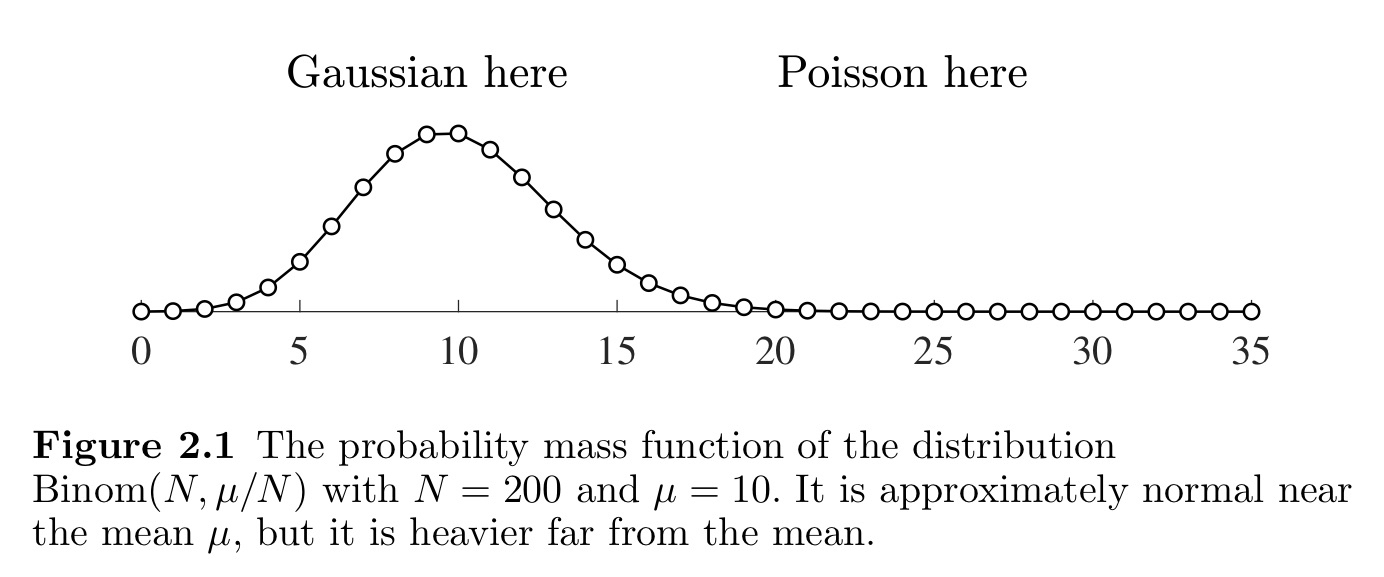
\includegraphics[width=0.8\textwidth]{Chapter 2/fig2-1.png}
\end{center}
\end{remark}


\subsection{Application: Median-of-means Estimator}
In data science, estimates are made using data frequently. Perhaps the most basic example is estimating 
the mean. Let $X$ be a random variable with mean $\mu$ (representing a population). Let $X_1, \dots, X_N$ 
be independent copies of $X$ (representing a sample). We want an estimator $\Hat{\mu}(X_1, \dots, X_N)$ 
to satisfy $\Hat{\mu} \approx \mu$ with high probability.


\subsection{Application: Degrees of Random Graphs}


\subsection{Subgaussian Distributions}

